\hypertarget{group__Fetch}{\section{Fetch}
\label{group__Fetch}\index{Fetch@{Fetch}}
}


Tools for fetching tests.  


Collaboration diagram for Fetch\-:
\nopagebreak
\begin{figure}[H]
\begin{center}
\leavevmode
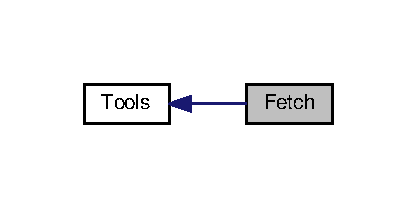
\includegraphics[width=200pt]{group__Fetch}
\end{center}
\end{figure}
Tools for fetching tests. \hypertarget{group__Fetch_AlreadyInstalled}{}\subsection{Already\-Installed}\label{group__Fetch_AlreadyInstalled}
No-\/op plugin for using existing middleware installation 
\begin{DoxyParams}{Parameters}
{\em exec} & Executable that should be in path \\
\hline
{\em module} & Modules (or lmod modules) to be loaded for accessing this package\\
\hline
\end{DoxyParams}
\hypertarget{group__Fetch_Git}{}\subsection{Git}\label{group__Fetch_Git}
Plugin for getting software via \hyperlink{namespaceGit}{Git} 
\begin{DoxyParams}{Parameters}
{\em module} & Modules (or lmod modules) to be loaded for accessing this package \\
\hline
{\em url} & U\-R\-L to access the repository \\
\hline
{\em username} & Username required for accessing the repository \\
\hline
{\em password} & Password required for that user to access the repository \\
\hline
{\em pwfile} & File where password can be found \\
\hline
{\em branch} & Branch (if not master) to be downloaded \\
\hline
{\em pr} & Pull request to be downloaded \\
\hline
{\em subdir} & Subdirectory of interest in repository\\
\hline
\end{DoxyParams}
\hypertarget{group__Fetch_OMPI_Snapshot}{}\subsection{O\-M\-P\-I\-\_\-\-Snapshot}\label{group__Fetch_OMPI_Snapshot}
Plugin for getting software via O\-M\-P\-I Nightly tarballs 
\begin{DoxyParams}{Parameters}
{\em url} & U\-R\-L to access the O\-M\-P\-I nightly tarball (e.\-g. \href{https://www.open-mpi.org/nightly/v2.x}{\tt https\-://www.\-open-\/mpi.\-org/nightly/v2.\-x}) \\
\hline
{\em version\-\_\-file} & optional file containing name of most recent tarball version tested \\
\hline
{\em mpi\-\_\-name} & optional name for the O\-M\-P\-I snapshot tarball \\
\hline
\end{DoxyParams}
